\documentclass[t]{beamer}
\usepackage{amsmath,amssymb}
\usepackage{mathrsfs} % for \mathscr
\usepackage{calc}
\usepackage[nomessages]{fp}
\usepackage{tikz,amsmath,amssymb}
%\usepackage[showframe]{geometry}
\usepackage{tkz-euclide} 
\usetikzlibrary{calc,arrows,decorations.markings, patterns}
\usepackage{quiver}
\usepackage[english]{babel}

\usepackage{tikz}
\usepackage{tikz-cd}

\usepackage{amsthm}
\usepackage[all]{xy}
\usepackage{ stmaryrd }
\usepackage{ mathrsfs }
\theoremstyle{plain} 
\newtheorem{scholie}{Scholie}
\usepackage{epsfig}
\usepackage{lmodern}
\usepackage{eurosym}
\usepackage{graphicx}
\usepackage{enumitem}
\usepackage{amsbsy}
\usepackage{rotating}
\usepackage[noabbrev,capitalise]{cleveref}
\usepackage{float}
\usepackage{stmaryrd}


% =========================
% Beamer Style (no content changes)
% =========================

% Fonts & micro-typography
\usepackage[T1]{fontenc}
\usepackage{microtype}
\usefonttheme{professionalfonts} % you already use lmodern; keep pro fonts
\setbeamerfont{frametitle}{size=\Large,series=\bfseries}
\setbeamerfont{framesubtitle}{size=\large}
\setbeamerfont{normal text}{size=\large} % slightly larger base for talk rooms
\setbeamerfont{block title}{series=\bfseries}
\setbeamerfont{footnote}{size=\scriptsize}

% Top alignment, margins, nav
\setbeamersize{text margin left=8mm,text margin right=8mm}
\setbeamertemplate{navigation symbols}{} % no nav buttons
% All frames are already top-aligned via \documentclass[t]{beamer}

% Structure & colors (use your palette)
\setbeamercolor{structure}{fg=darkcerulean}
\setbeamercolor{frametitle}{fg=darkcerulean}
\setbeamercolor{framesubtitle}{fg=darkcerulean}
\setbeamercolor{normal text}{fg=black,bg=white}

% Blocks (definition/theorem/alert styles)
\setbeamercolor{block title}{bg=darkcerulean!8, fg=darkcerulean}
\setbeamercolor{block body}{bg=darkcerulean!2}
\setbeamercolor{block title alerted}{bg=lava!10, fg=lava!90!black}
\setbeamercolor{block body alerted}{bg=lava!3}
\setbeamercolor{block title example}{bg=jade!12, fg=darkgreen}
\setbeamercolor{block body example}{bg=jade!4}

% Theorems (you already set fonts; here we unify colors)
\setbeamercolor{theorem title}{fg=darkcerulean}
\setbeamercolor{theorem body}{fg=black}

% Itemize/Enumerate spacing & symbols (uniform)
\usepackage{enumitem}
\setlist[itemize]{leftmargin=1.2em,itemsep=2mm,topsep=1mm}
\setlist[enumerate]{leftmargin=1.4em,itemsep=2mm,topsep=1mm}
\setbeamertemplate{itemize item}{\raisebox{0.15ex}{\tiny$\blacksquare$}}
\setbeamertemplate{itemize subitem}{\tiny$\bullet$}
\setbeamertemplate{itemize subsubitem}{\tiny$\circ$}

% Math display spacing (tighter for slides)
\AtBeginDocument{%
  \abovedisplayskip=8pt plus 2pt minus 2pt
  \belowdisplayskip=8pt plus 2pt minus 2pt
  \abovedisplayshortskip=6pt plus 2pt minus 2pt
  \belowdisplayshortskip=6pt plus 2pt minus 2pt
}

% Captions (if you use them)
\setbeamerfont{caption}{size=\small}
\setbeamercolor{caption name}{fg=darkcerulean}

% Frametitle underline rule (subtle)
\addtobeamertemplate{frametitle}{}{%
  \vspace{-0.2em}%
  \par\noindent\color{darkcerulean!35}\rule{\linewidth}{0.4pt}\par\vspace{-0.4em}%
}

% Clean footline (Title • Author • slide#/total)
\makeatletter
\defbeamertemplate*{footline}{custom thin}{%
  \leavevmode%
  \hbox{%
    \begin{beamercolorbox}[wd=.34\paperwidth,ht=2.5ex,dp=1ex,left]{author in head/foot}%
      \hspace{1.2em}\usebeamerfont{author in head/foot}\insertshorttitle
    \end{beamercolorbox}%
    \begin{beamercolorbox}[wd=.32\paperwidth,ht=2.5ex,dp=1ex,center]{title in head/foot}%
      \usebeamerfont{title in head/foot}\insertshortauthor
    \end{beamercolorbox}%
    \begin{beamercolorbox}[wd=.34\paperwidth,ht=2.5ex,dp=1ex,right]{date in head/foot}%
      \usebeamerfont{date in head/foot}\insertframenumber{} / \inserttotalframenumber\hspace{1.2em}
    \end{beamercolorbox}%
  }%
}
\setbeamertemplate{footline}[custom thin]
\makeatother

% XY & TikZ arrows unified
\SelectTips{cm}{} % nicer Computer Modern tips for xy
\xyoption{tips}
\tikzset{>=stealth, every picture/.style={line cap=round,line join=round}}
% (Your internal small posets still use ">= angle 60"; that's fine—this only sets a default.)

% Hyperref (keep your colors; make links subtle but consistent)
\hypersetup{
  colorlinks=true,
  linkcolor=darkcerulean,
  citecolor=jade,
  urlcolor=bleudefrance,
  pdfpagemode=UseNone
}



\usepackage{stackengine,scalerel}
\stackMath
\def\Tleq{\ThisStyle{\mathrel{%
  \stackinset{r}{.7pt+.15\LMpt}{t}{.1\LMpt}{\rule{.4pt}{1.1\LMex+.2ex}}{\SavedStyle\leqslant}%
}}}

\def\TleqE{\ThisStyle{\mathrel{%
  \stackinset{r}{6pt+.15\LMpt}{t}{.1\LMpt}{\rule{.4pt}{1.1\LMex+.2ex}}{\SavedStyle\leqslant_\mathcal{E}}%
}}}

\def\TleqEunder{\ThisStyle{\mathrel{%
  \stackinset{r}{5.4pt+.15\LMpt}{t}{.1\LMpt}{\rule{.4pt}{1.1\LMex+.2ex}}{\SavedStyle\leqslant_\mathcal{E}}%
}}}

\def\TldotE{\ThisStyle{\mathrel{%
  \stackinset{r}{6pt+.15\LMpt}{t}{.1\LMpt}{\rule{.4pt}{1.1\LMex+.2ex}}{\SavedStyle\lessdot_\mathcal{E}}%
}}}

\def\TldotEunder{\ThisStyle{\mathrel{%
  \stackinset{r}{5.4pt+.15\LMpt}{t}{.1\LMpt}{\rule{.4pt}{1.1\LMex+.2ex}}{\SavedStyle\lessdot_\mathcal{E}}%
}}}

\definecolor{midnightblue}{rgb}{0.1, 0.1, 0.44}
\definecolor{plum}{rgb}{0.56, 0.27, 0.52}
\definecolor{Plum}{rgb}{0.56, 0.27, 0.52}
\definecolor{patriarch}{rgb}{0.5, 0.0, 0.5}
\definecolor{darkgreen}{rgb}{0.0, 0.2, 0.13}
\definecolor{darkcerulean}{rgb}{0.03, 0.27, 0.49}
\definecolor{jade}{rgb}{0.0, 0.66, 0.42}
\definecolor{bleudefrance}{rgb}{0.19, 0.55, 0.91}
\definecolor{lava}{rgb}{0.81, 0.06, 0.13}

\hypersetup{
	colorlinks=true,
	linkcolor=darkcerulean,
	citecolor=jade,
	filecolor=magenta,      
	urlcolor=cyan,
	pdfpagemode=FullScreen,
}

\newcommand{\ccong}{\mathbin{\rotatebox[origin=c]{90}{$\cong$}}}
\newcommand{\rep}{\operatorname{rep}}
\newcommand{\Cat}{\operatorname{Cat}}
\newcommand{\Int}{\operatorname{Int}}
\newcommand{\GenJF}{\operatorname{GenJF}}
\newcommand{\GenRep}{\operatorname{GenRep}}
\newcommand{\JF}{\operatorname{JF}}
\newcommand{\vJF}{\pmb{\operatorname{JF}}}
\newcommand{\adj}{\operatorname{adj}}
\newcommand{\add}{\operatorname{add}}
\newcommand{\Ker}{\operatorname{Ker}}
\newcommand{\Coker}{\operatorname{Coker}}
\newcommand{\Hom}{\operatorname{Hom}}
\newcommand{\Id}{\operatorname{Id}}
\newcommand{\IIm}{\operatorname{Im}}
\newcommand{\mult}{\operatorname{mult}}
\newcommand{\diag}{\operatorname{diag}}
\newcommand{\op}{\operatorname{op}}
\newcommand{\ind}{\operatorname{ind}}
\newcommand{\refl}{\operatorname{refl}}
\newcommand{\GK}{\operatorname{\mathsf{GK}}}
\newcommand{\NEnd}{\operatorname{\mathsf{N}End}}
\newcommand{\wt}{\operatorname{\mathsf{wt}}}
\newcommand{\End}{\operatorname{End}}
\newcommand{\Ext}{\operatorname{Ext}}
\newcommand{\supp}{\operatorname{supp}}
\newcommand{\vdim}{\operatorname{\pmb{\dim}}}
\newcommand{\Vect}{\operatorname{Vect}}
\newcommand{\Adds}{\operatorname{AddS}}
\newcommand{\Ind}{\operatorname{Ind}}
\newcommand{\Supp}{\operatorname{Supp}}
\newcommand{\rev}{\operatorname{rev}}
\newcommand{\C}{\mathbf{C}}
\newcommand{\F}{\mathbf{F}}
\renewcommand{\L}{\mathbf L}
\newcommand{\R}{\mathbf R}
\newcommand{\A}{\mathbf A}
\newcommand{\B}{\mathbf B}
\newcommand{\E}{\mathbf E}
\newcommand{\intp}{\operatorname{\mathbf{int}}}
\newcommand{\RSK}{\operatorname{RSK}}
\newcommand{\tog}{\operatorname{tog}}
\newcommand{\compl}{\operatorname{compl}}
\newcommand{\eff}{\operatorname{eff}}
\newcommand{\RPP}{\operatorname{RPP}}
\newcommand{\Tilt}{\operatorname{Tilt}}
\renewcommand{\Box}{\operatorname{Box}}
\newcommand{\Fer}{\operatorname{Fer}}
\newcommand{\SSYT}{\operatorname{SSYT}}
\newcommand{\SYT}{\operatorname{SYT}}
\newcommand{\AR}{\operatorname{AR}}
\newcommand{\Mult}{\operatorname{Mult}}
\newcommand{\Mat}{\operatorname{Mat}}
\newcommand{\GL}{\operatorname{GL}}
\newcommand{\vGL}{\pmb{\operatorname{GL}}}
\newcommand{\pdim}{\operatorname{pdim}}
\newcommand{\proj}{\operatorname{proj}}
\newcommand{\inj}{\operatorname{inj}}
\newcommand{\Gen}{\operatorname{Gen}}
\newcommand{\Rad}{\operatorname{Rad}}
\newcommand{\Sub}{\operatorname{Sub}}
\newcommand{\GS}{\operatorname{GS}}
\newcommand{\SG}{\operatorname{SG}}
\newcommand{\opC}{\operatorname{\pmb{\mathscr{C}}}}
\newcommand{\opJ}{\operatorname{\pmb{\mathscr{J}}}}
\newcommand{\opT}{\operatorname{\pmb{T}}}
\renewcommand\qedsymbol{$\blacksquare$}
\newcommand{\epip}{ \xymatrix{   \ar@{-->>}[r] &  \\} }
\newcommand{\epi}{ \xymatrix{   \ar@{>>}[r] &  \\} }
\newcommand{\p}{ \xymatrix{   \ar@{-->}[r] &  \\} }
\newcommand{\Exact}{\pmb{\operatorname{Ext}}}
\newcommand{\llrr}[1]{\llbracket #1 \rrbracket}
\AtEndEnvironment{ex}{\renewcommand{\qedsymbol}{}}
\newcommand{\CK}{\mathrm{CK}}
\setbeamerfont{theorem body}{series=\normalfont,shape=\itshape} % italics like article
\setbeamerfont{theorem title}{series=\bfseries} % bold title
\usepackage[all]{xy} % <-- xy-pic
\usefonttheme{professionalfonts} 
\usepackage{lmodern}      % Computer Modern Latin Modern
\newcommand{\SecRomanUp}[1]{\MakeUppercase{\romannumeral #1}}
\setbeamertemplate{subsection in toc}{} % hide subsections (optional, cleaner)
\setbeamerfont{section in toc}{size=\large}
\setbeamertemplate{section in toc}{%
  \vspace{3pt}%
  \textbf{\SecRomanUp{\inserttocsectionnumber}.}\hspace{0.6em}\inserttocsection\par
}

\setbeamertemplate{footline}{}
\title{Exact Structures and Maximal Canonically Jordan Recoverable Subcategories\\for Modules over Type \(A\) Algebras}
\author{Sunny Roy}
\institute{Département de mathématiques, Université de Sherbrooke}
\date{October 23\textsuperscript{th}}

\begin{document}
\AtBeginSection[]{
  \begin{frame}{Plan}
    \tableofcontents[currentsection]
  \end{frame}
}




% === TITLE SLIDE ===
\begin{frame}
  \titlepage
  \centering

  35\textsuperscript{th} Meeting on the Representation Theory of Algebras\\
  and Related Topics (RTA 2025, Sherbrooke, Québec)\\
  October 23 – 25, 2025\\[1em]
  \vfill
  \small
  Based on joint work with Benjamin Dequêne\\
  (arXiv:2509.25012v2)
\end{frame}
% After \frame{\titlepage}
\begin{frame}{Plan}
  \tableofcontents[pausesections]
\end{frame}

\section{Motivation: Jordan Recoverability and Canonical Jordan Recoverability}
\begin{frame}{Motivation}
  In representation theory, we often seek invariants that classify objects
  up to isomorphism.

\pause

  \medskip
  The \textbf{Jordan form} is one of the simplest and most classical invariants
  attached to endomorphisms. It encodes essential structural information.

\pause
  \medskip

   \textbf{Question} : Can a representation be recovered from the Jordan forms of its nilpotent endomorphisms?
\pause

  \medskip
 In recent work, \textbf{Garver–Patrias–Thomas} (2018–2022)
introduced and developed the notions of
\emph{Jordan recoverability (JR)} and
\emph{canonical Jordan recoverability (CJR)}.
These ideas were later expanded by \textbf{Dequêne} (2022–2024).
\end{frame}

\begin{frame}{Settings}

\begin{itemize}
  \item[\large$\bullet$] $K$ is an algebraically closed field.
  \pause
  \item[\large$\bullet$] $Q$ is a \textbf{Dynkin quiver} with no relations.
  \pause
  \item[\large$\bullet$] $\rep(Q)$ denotes the category of finite-dimensional left $KQ$-modules.
  \pause
  \item[\large$\bullet$] $\mathscr{A}$ will denote a \textbf{hereditary abelian category}.
  \pause
  \item[\large$\bullet$] All subcategories are assumed \textbf{full, closed under finite direct sums, and under direct summands.}
\end{itemize}

\end{frame}


\begin{frame}{Jordan Form for Representations}
  
    \emph{Let $E=(E_q,E_\alpha)\in \mathrm{rep}Q$ and 
    $N=(N_q)_{q\in Q_0}\in \mathrm{NEnd}(E)$.}
    Each $N_q$ is a nilpotent endomorphism of $E_q$.
  

  \begin{block}{Definition}
    The \textbf{Jordan form} of $N_q$ is the partition
    $JF(N_q)\vdash \dim(E_q)$ recording its Jordan block sizes.
    Define the tuple
    \[
      JF(N) \;=\; (JF(N_q))_{q\in Q_0},
    \]
    which describes the block structure of $N$ at each vertex.
  \end{block}
\end{frame}

\begin{frame}{The Generic Jordan Form Invariant}
  
    \emph{Fix $E\in \mathrm{rep}Q$.
    For $N=(N_q)_{q\in Q_0}\in \mathrm{NEnd}(E)$, set
    \[
      JF(N)=(JF(N_q))_{q\in Q_0}.
    \]
 

  \pause
  \begin{block}{Definition [GPT23]}
      
      The \textbf{generic Jordan form} of $E$ is the maximal value (with respect to dominance order):
            \[
              \GenJF(E)\;=\; \max_{N\in \mathrm{NEnd}(E)} JF(N).
            \]
    
  \end{block}
  }
  \textbf{Question} : Is this invariant complete?
\end{frame}


\begin{frame}{Jordan Recoverability}
  \begin{block}{Definition [GPT23]}
    \emph{Let $\mathscr{C}\subseteq \mathrm{rep}Q$ be a subcategory.}
    We say that $\mathscr{C}$ is \textbf{Jordan recoverable (JR)} if
    \[
      E \simeq F 
      \;\Longleftrightarrow\;
      \GenJF(E)=\GenJF(F)
      \qquad\text{for all } E,F\in \mathscr{C}.
    \]
  \end{block}

  \begin{block}{Remark}
    The generic Jordan form $\GenJF$ is a \emph{complete invariant} on $\mathscr{C}$.
  \end{block}
\end{frame}


\begin{frame}{Canonical Jordan Recoverability (CJR)}
  \emph{ \begin{block}{Definition [GPT23]}
   Let $\mathscr{C}\subseteq \mathrm{rep}Q$
    We say $\mathscr{C}$ is \textbf{canonically Jordan recoverable (CJR)} if for every
    $X\in \mathscr{C}$ there exists a dense open set (in the Zariski sense)
    $\Omega \subseteq \mathrm{rep}(Q,\GenJF(X))$ such that for all $Y\in \Omega$,
    $Y\simeq X$.
  \end{block}

  \pause
  \begin{block}{Maximal CJR subcategory}
    A CJR subcategory $\mathscr{C}$ is \textbf{maximal} if it is not properly contained
    in any larger CJR subcategory of $\mathrm{rep}Q$, i.e.
    \[
      \forall\,\mathcal{D}\supsetneq \mathscr{C},\quad \mathcal{D}\ \text{is not CJR.}
    \]
    
  \end{block}
  }
\end{frame}

\begin{frame}{Example on $A_2$: JR but not CJR}
  
    Assume $Q: 1\to 2$ and let $\mathscr{C}=\mathrm{add}(S_1,S_2)\subseteq \mathrm{rep}(Q)$.
    Every $E\in \mathscr{C}$ has the form
    \[
      E=K^a \xrightarrow{0} K^b .
    \]
  

  \pause
 \textbf{Generic Jordan form}
    \[
      \GenJF(E)=\bigl((a),(b)\bigr).
    \]
    Hence $\mathscr{C}$ is \textbf{JR}:
    \emph{$E\simeq F \iff \GenJF(E)=\GenJF(F)$ in $\mathscr{C}$.}
  
\bigskip
  \pause
  \textbf{Open sets with generic Jordan form \((1,1)\).}
  
  \smallskip
  
    Consider $S_1\oplus S_2 \cong K \xrightarrow[]{0} K$.
    Any dense open $U \subset \mathrm{rep}_K(Q,(1,1))$ contains representations
    $K \xrightarrow[]{\lambda} K \cong P_1$ with $\lambda\neq 0$.
  
\bigskip
  \pause
  
    We have $\GenJF(S_1\oplus S_2)=((1),(1))=\GenJF(P_1)$ with $P_1\in U$, but
    $S_1\oplus S_2 \ncong P_1$. Hence $\mathscr{C}$ is \textbf{not CJR}.
  
\end{frame}


\begin{frame}{Maximal CJR subcategories in type $A_n$}

    \emph{Let $Q$ be a quiver of type $A_n$.
 

  \pause
  \begin{block}{Proposition}
    If $\mathscr{C}\subseteq \mathrm{rep}Q$ is a maximal canonically Jordan
    recoverable subcategory, then:
    \pause
    \begin{itemize}
      \item[(a)] $\mathscr{C}$ is extension-closed;
      \pause
      \item[(b)] $\mathscr{C}$ always contains a tilting representation.
    \end{itemize}
  \end{block}

  \pause
  \begin{block}{Theorem [Deq23a]}
    A subcategory $\mathscr{C}\subseteq \mathrm{rep}(Q)$ is canonically Jordan
    recoverable if and only if every non-split short exact sequence
    \[
      0 \longrightarrow X \longrightarrow Y \longrightarrow Z \longrightarrow 0
    \]
    with $X,Z\in \mathscr{C}$, $Y \notin \ind(\mathrm{rep}\,Q)$.
  \end{block}
  }
\end{frame}
\section{The Diamond Exact Structure \texorpdfstring{$\mathcal{E}_\diamond$}{E-diamond}}
% ------------------------
% ES1 + ES2 + ES3 + ES4
% ------------------------
\begin{frame}{Exact Structures}
\begin{block}{Definition}
  A collection $\mathcal{E}$ of short exact sequences in $\mathscr{A}$ 
  is an exact structure on $\mathscr{A}$ whenever $\mathcal{E}$ satisfies 
  the following axioms:
  \end{block}
  
\pause

  \begin{itemize}
    \item[(ES1)] All the split short exact sequences are in $\mathcal{E}$;
\pause    
    \item[(ES2)] The collection of $\mathcal{E}$-monomorphisms and the one of $\mathcal{E}$-epimorphisms are
                both closed under compositions;
\pause
    \item[(ES3)] $\mathcal{E}$ is closed under the pushouts and pullbacks along any morphism: that is, for any short exact sequence in $\mathcal{E}$: 
  \vspace{-3em}
\pause
\begin{columns}[t]
  % Left column: Pushout
  \begin{column}{0.48\textwidth}
    \begin{center}
      \[
      \xymatrix@C=6mm@R=3mm{
      0 \ar[r] & X\; \ar@{>->}[r]^{f} \ar[d]_{h} 
               & Y \ar@{->>}[r] \ar[d] 
               & Z \ar[r] \ar@{=}[d] & 0 \\
      0 \ar[r] & D \;\ar@{>->}[r] 
               & PO \ar@{->>}[r] 
               & Z \ar[r] & 0
      }
      \]
      \textbf{(ES3-I) Pushouts} \\
      $\mathcal{E}$ is closed under pushouts.
    \end{center}
  \end{column}
\pause
  % Right column: Pullback
  \begin{column}{0.48\textwidth}
    \begin{center}
      \[
      \xymatrix@C=6mm@R=3mm{
      0 \ar[r] & X \; \ar@{>->}[r] \ar@{=}[d] 
               & Y \ar@{->>}[r]^{g}  
               & Z \ar[r] & 0 \\
      0 \ar[r] & X \; \ar@{>->}[r] 
               & PB \ar[u] \ar@{->>}[r] 
               & F \ar[r] \ar[u]^{h'} & 0
      }
      \]
      \textbf{(ES3-II) Pullbacks} \\
      $\mathcal{E}$ is closed under pullbacks.
    \end{center}
  \end{column}
\end{columns}

  \end{itemize}
\end{frame}





\begin{frame}{Exact Categories}
  \begin{block}{Definition}
    Let $\mathcal{E}$ be an exact structure on $\mathscr{A}$.  
    The pair $(\mathscr{A},\mathcal{E})$ is called an \textbf{exact category}.
  \end{block}
\pause
  \bigskip

  \begin{block}{Example of Exact Structures}
    \begin{itemize}
      \item $\mathcal{E}_{\max}$ : the \emph{maximal exact structure}, containing all short exact sequences.
      \pause
      \item $\mathcal{E}_{\min}$ : the \emph{minimal exact structure}, containing only the split short exact sequences.
    \end{itemize}
  \end{block}
\end{frame}


\begin{frame}{Short Exact Sequences in Type $A_n$}
\begin{theorem}
Let $Q$ be an $A_n$ type quiver.  
For a non-split exact sequence
\[
0 \longrightarrow D \longrightarrow E \longrightarrow F \longrightarrow 0,
\qquad D,F \in \ind(\rep Q),
\]
exactly one of the following holds:
\pause
\begin{enumerate}[label=(\alph*)]
  \item $E \in \ind(\rep Q)$, 
\pause
  \item $E \cong E_1 \oplus E_2$ with $E_1,E_2 \in \ind(\rep Q)$.
\end{enumerate}
\smallskip
\end{theorem}
\pause
In case (b) we call it a \textbf{diamond exact sequence}.

\end{frame}

% Preamble (ensure paper-like fonts)
% \usefonttheme{professionalfonts}
% \usepackage{lmodern}
% \usepackage{amsmath,amssymb,mathrsfs}

% ---------- Definition: E_diamond ----------
\begin{frame}{The Diamond Exact Structure \(\mathcal{E}_\diamond\)}

\begin{block}{Definition}
Let \(Q\) be an \(A_n\) type quiver.  
We define the collection of short exact sequences
\(\mathcal{E}_{\diamond}\) given by the additive bifunctor
\(\mathcal{E}_\diamond(-,-)\), uniquely determined by
\[
\mathcal{E}_\diamond(N,M)
= \bigl\{\, \eta \in \Ext^1(N,M) \;\big|\;
\eta \text{ splits or diamond exact sequence}\,\bigr\}
\]
for \(M,N \in \ind(\rep Q)\) indecomposable.
\end{block}

\pause

\begin{block}{Proposition [Brüstle–Hanson–R.–Schiffler, 2024]}
Let \(n \in \mathbb{N}^*\) and \(Q\) be an \(A_n\) type quiver.  
Then \(\mathcal{E}_{\diamond}\) is an exact structure on \(\mathscr{A}=\rep(Q)\).
\end{block}

\end{frame}

\begin{frame}{Restatement of Theorem on CJR subcategories}
\begin{theorem}
Let $Q$ be an $A_n$ type quiver.  
A subcategory $\mathscr{C} \subseteq \rep(Q)$ is canonically Jordan recoverable  
if and only if $\mathscr{C}$ is $\mathcal{E}_\diamond$-adapted.
\end{theorem}

\pause
\bigskip

\textbf{Remark.} 
$\mathscr{C}$ is maximal canonically Jordan recoverable if any subcategory $\mathscr{D}  \supset \mathscr{C}$ is not $\mathcal{E}_\diamond$-adapted.  
\end{frame}

\section{The \texorpdfstring{$\GS_\mathcal{E}$}{GS(E)} Operator \& Properties\\ \normalsize (First Main Theorem)}

\begin{frame}{The $\Gen_\mathcal{E}$ and $\Sub_\mathcal{E}$ Operators}
Let $(\mathscr{A},\mathcal{E})$ be an exact category.

\smallskip

\emph{\begin{block}{Definition.} 
For a subcategory $\mathscr{C} \subseteq \mathscr{A}$, we define the subcategories:
\pause
\begin{enumerate}[label=(\alph*), itemsep=2mm] \item $\Gen_\mathcal{E}(\mathscr{C}) = \bigl\{C \in \mathscr{A} \;\big|\; g : Y \twoheadrightarrow C, \,~Y \in \mathscr{C},~ g \text{ an $\mathcal{E}$-epi}\bigr\};$ 
\pause
\item $\Sub_\mathcal{E}(\mathscr{C}) = \bigl\{K \in \mathscr{A} \;\big|\; f:K \rightarrowtail Y,~Y \in \mathscr{C},~ f \text{ an $\mathcal{E}$-mono}\bigr\}.$ \end{enumerate}
\end{block}
\pause
\bigskip
For an object $M \in \mathscr{A}$, we set
\(\Gen_\mathcal{E}(M) = \Gen_\mathcal{E}(\add(M))\),
\(\Sub_\mathcal{E}(M) = \Sub_\mathcal{E}(\add(M))\).
}
\end{frame}





\begin{frame}{The $\GS_\mathcal{E}$ Construction}
\emph{\begin{block}{Defintion} 
Let $\mathscr{C} \subseteq \mathscr{A}$ be a subcategory.
\pause
\begin{enumerate}[label=(\alph*), itemsep=2mm]
  \item Set $\GS_\mathcal{E}^0(\mathscr{C}) = \mathscr{C}$.
\pause
  \item For $i \geq 1$, define
  \[
    \GS_\mathcal{E}^i(\mathscr{C})
    = \add\!\Bigl(\Gen_\mathcal{E}(\GS_\mathcal{E}^{i-1}(\mathscr{C}))
    \;\cup\; \Sub_\mathcal{E}(\GS_\mathcal{E}^{i-1}(\mathscr{C}))\Bigr).
  \]
\end{enumerate}

\end{block}
\pause
\smallskip
\textbf{Remark.} $(\GS_\mathcal{E}^i(\mathscr{C}))_{i \in \mathbb{N}}$ is an increasing sequence of subcategories of $\mathscr{A}$.
}




\end{frame}



\begin{frame}{The $\GS_\mathcal{E}$ Construction}

\emph{
\begin{block} {Definition}
The $\GS_\mathcal{E}$-operator is defined by
\[
\GS_\mathcal{E}(\mathscr{C})
= \varinjlim_{i \in \mathbb{N}} \GS_\mathcal{E}^i(\mathscr{C})
= \bigcup_{i \in \mathbb{N}} \GS_\mathcal{E}^i(\mathscr{C}).
\]
\pause
Equivalently, $\GS_\mathcal{E}(\mathscr{C})$ is the smallest subcategory of $\mathscr{A}$ 
that contains $\mathscr{C}$ and is closed under both $\Gen_\mathcal{E}$ and $\Sub_\mathcal{E}$.
    
\end{block}

\pause
\smallskip
For an object $M \in \mathscr{A}$, we set
$\GS_\mathcal{E}(M) = \GS_\mathcal{E}(\add(M))$.

}

\end{frame}


\begin{frame}{$\GS^0_\mathcal{E_\diamond}(\protect
\begin{tikzpicture}[baseline={(0,-.1)}]
        \node[circle, line width=0.2mm, double, fill=lava!20,minimum size=1em,draw] at (0,0){$ $};
    \end{tikzpicture}) = \add(\protect
\begin{tikzpicture}[baseline={(0,-.1)}]
        \node[circle, line width=0.2mm, double, fill=lava!20,minimum size=1em,draw] at (0,0){$ $};
    \end{tikzpicture})$ }


\centering
    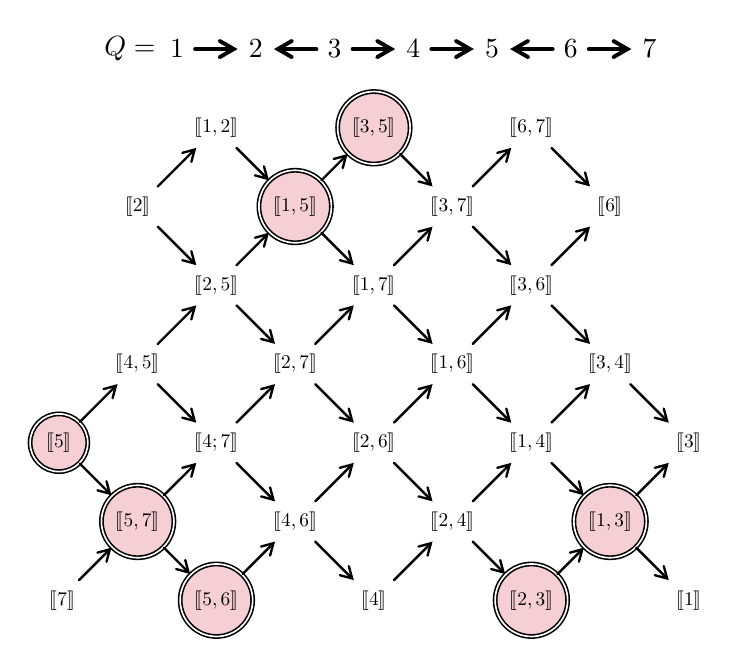
\begin{tikzpicture}
				\begin{scope}[line width=.5mm,->, >= angle 60]
                    \node at (-.6,0){$Q=$};
					\node (a) at (0,0){$1$};
					\node (b) at (1,0){$2$};
					\node (c) at (2,0){$3$};
					\node (d) at (3,0){$4$};
                    \node (e) at (4,0){$5$};
                    \node (f) at (5,0){$6$};
                    \node (g) at (6,0){$7$};
					\draw (a) -- (b);
					\draw (c) -- (b);
					\draw (c) -- (d);
                    \draw (d) -- (e);
                    \draw (f) -- (e);
                    \draw (f) -- (g);
				\end{scope}
                \begin{scope}[yshift=-2cm, xshift=-.5cm, line width=.3mm, ->, >= angle 60]
					\node (2) at (0,0){\scalebox{.7}{$\llrr{2}$}};
					\node (12) at (1,1){\scalebox{.7}{$\llrr{1,2}$}};
					\node (2345) at (1,-1){\scalebox{.7}{$\llrr{2,5}$}};
					\node (45) at (0,-2){\scalebox{.7}{$\llrr{4,5}$}};
                    \node[circle,line width=0.2mm,double,fill=lava!20,draw] (5) at (-1,-3){\scalebox{.7}{$\llrr{5}$}};
                    \node[circle,line width=0.2mm,double,fill=lava!20,draw] (567) at (0,-4){\scalebox{.7}{$\llrr{5,7}$}};
                    \node (7) at (-1,-5){\scalebox{.7}{
							$\llrr{7}$}};
                    \node (56)[circle,line width=0.2mm,double,fill=lava!20,draw] at (1,-5){\scalebox{.7}{$\llrr{5,6}$}
                                };
                     \node (4) at (3,-5){\scalebox{.7}{$\llrr{4}$}};
                     \node[circle,line width=0.2mm,double,fill=lava!20,draw] (23) at (5,-5){\scalebox{.7}{$\llrr{2,3}$}};
                    \node (1) at (7,-5){\scalebox{.7}{$\llrr{1}$}};
                    \node (456) at (2,-4){\scalebox{.7}{$\llrr{4,6}$}};
                    \node (234) at (4,-4){\scalebox{.7}{$\llrr{2,4}$}};
                     \node[circle,line width=0.2mm,double,fill=lava!20,draw] (123) at (6,-4){\scalebox{.7}{$\llrr{1,3}$}};
                     \node (4567) at (1,-3){\scalebox{.7}{$\llrr{4;7}$}};
                     \node (23456) at (3,-3){\scalebox{.7}{$\llrr{2,6}$}};
                     \node (1234) at (5,-3){\scalebox{.7}{$\llrr{1,4}$}};
                     \node (3) at (7,-3){\scalebox{.7}{$\llrr{3}$}};
					\node[circle,line width=0.2mm, double,fill=lava!20,draw] (12345) at (2,0){\scalebox{.7}{$\llrr{1,5}$}};
					\node (234567) at (2,-2){\scalebox{.7}{$\llrr{2,7}$}};
                    \node (123456) at (4,-2){\scalebox{.7}{$\llrr{1,6}$}};
					\node (34) at (6,-2){\scalebox{.7}{$\llrr{3,4}$}};
					\node (1234567) at (3,-1){\scalebox{.7}{$\llrr{1,7}$}};
                    \node (3456) at (5,-1){\scalebox{.7}{$\llrr{3,6}$}};
                    \node (34567) at (4,0){\scalebox{.7}{$\llrr{3,7}$}};
                    \node (6) at (6,0){\scalebox{.7}{$\llrr{6}$}};
                    \node[circle,line width=0.2mm,double,fill=lava!20,draw] (345) at (3,1){\scalebox{.7}{$\llrr{3,5}$}};
                    \node (67) at (5,1){\scalebox{.7}{$\llrr{6,7}$}};
					\draw (2) -- (12);
					\draw (2) -- (2345);
					\draw (45) -- (2345);
					\draw (12) -- (12345);
					\draw (2345) -- (12345);
					\draw (2345) -- (234567);
                    \draw (12345) -- (345);
                    
                    
                    \draw (5) -- (45);
                    \draw (7) -- (567);
                    \draw (567) -- (4567);
                    \draw (4567) -- (234567);
                    \draw (234567) -- (1234567);
                    \draw (1234567) -- (34567);
                    \draw (34567) -- (67);
                    \draw (56) -- (456);
                    \draw (456) -- (23456);
                    \draw (23456) -- (123456);
                    \draw (123456) -- (3456);
                    \draw (3456) -- (6);
                    \draw (4) -- (234);
                    \draw (234) -- (1234);
                    \draw (1234) -- (34);
                    \draw (23) -- (123);
                    \draw (123) -- (3);
					
					\draw (5) -- (567);
                    \draw (567) -- (56);
                    \draw (45) -- (4567);
                    \draw (4567) -- (456);
                    \draw (456) -- (4);
                    \draw (234567) -- (23456);
                    \draw (23456) -- (234);
                    \draw (234) -- (23);
                    \draw (12345) -- (1234567);
                    \draw (1234567) -- (123456);
                    \draw (123456) -- (1234);
                    \draw (1234) -- (123);
                    \draw (123) -- (1);
                    \draw (345) -- (34567);
                    \draw (34567) -- (3456);
                    \draw (3456) -- (34);
                    \draw (34) -- (3);
                    \draw (67) -- (6);	
				\end{scope}
    \end{tikzpicture} 

\end{frame}

\begin{frame}{$\GS^1_\mathcal{E_\diamond}(\protect
\begin{tikzpicture}[baseline={(0,-.1)}]
        \node[circle, line width=0.2mm, double, fill=lava!20,minimum size=1em,draw] at (0,0){$ $};
    \end{tikzpicture})$}
    

\centering
    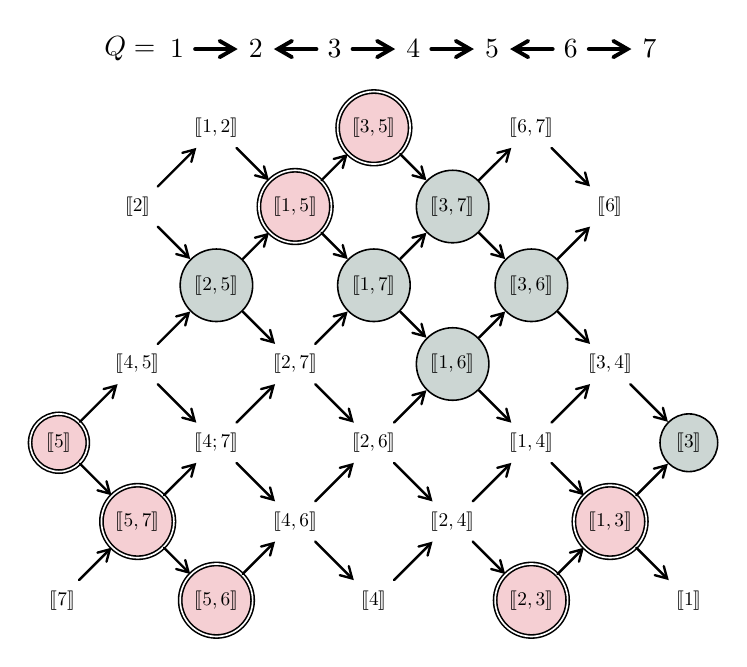
\begin{tikzpicture}
				\begin{scope}[line width=.5mm,->, >= angle 60]
                    \node at (-.6,0){$Q=$};
					\node (a) at (0,0){$1$};
					\node (b) at (1,0){$2$};
					\node (c) at (2,0){$3$};
					\node (d) at (3,0){$4$};
                    \node (e) at (4,0){$5$};
                    \node (f) at (5,0){$6$};
                    \node (g) at (6,0){$7$};
					\draw (a) -- (b);
					\draw (c) -- (b);
					\draw (c) -- (d);
                    \draw (d) -- (e);
                    \draw (f) -- (e);
                    \draw (f) -- (g);
				\end{scope}
                \begin{scope}[yshift=-2cm, xshift=-.5cm, line width=.3mm, ->, >= angle 60]
					\node (2) at (0,0){\scalebox{.7}{$\llrr{2}$}};
					\node (12) at (1,1){\scalebox{.7}{$\llrr{1,2}$}};
					\node[circle,line width=0.2mm,fill=darkgreen!20,draw] (2345) at (1,-1){\scalebox{.7}{$\llrr{2,5}$}};
					\node (45) at (0,-2){\scalebox{.7}{$\llrr{4,5}$}};
                    \node[circle,line width=0.2mm,double,fill=lava!20,draw] (5) at (-1,-3){\scalebox{.7}{$\llrr{5}$}};
                    \node[circle,line width=0.2mm,double,fill=lava!20,draw] (567) at (0,-4){\scalebox{.7}{$\llrr{5,7}$}};
                    \node (7) at (-1,-5){\scalebox{.7}{
							$\llrr{7}$}};
                    \node (56)[circle,line width=0.2mm,double,fill=lava!20,draw] at (1,-5){\scalebox{.7}{$\llrr{5,6}$}
                                };
                     \node (4) at (3,-5){\scalebox{.7}{$\llrr{4}$}};
                     \node[circle,line width=0.2mm,double,fill=lava!20,draw] (23) at (5,-5){\scalebox{.7}{$\llrr{2,3}$}};
                    \node (1) at (7,-5){\scalebox{.7}{$\llrr{1}$}};
                    \node (456) at (2,-4){\scalebox{.7}{$\llrr{4,6}$}};
                    \node (234) at (4,-4){\scalebox{.7}{$\llrr{2,4}$}};
                     \node[circle,line width=0.2mm,double,fill=lava!20,draw] (123) at (6,-4){\scalebox{.7}{$\llrr{1,3}$}};
                     \node (4567) at (1,-3){\scalebox{.7}{$\llrr{4;7}$}};
                     \node (23456) at (3,-3){\scalebox{.7}{$\llrr{2,6}$}};
                     \node (1234) at (5,-3){\scalebox{.7}{$\llrr{1,4}$}};
                     \node[circle,line width=0.2mm,fill=darkgreen!20,draw] (3) at (7,-3){\scalebox{.7}{$\llrr{3}$}};
					\node[circle,line width=0.2mm, double,fill=lava!20,draw] (12345) at (2,0){\scalebox{.7}{$\llrr{1,5}$}};
					\node (234567) at (2,-2){\scalebox{.7}{$\llrr{2,7}$}};
                    \node[circle,line width=0.2mm,fill=darkgreen!20,draw] (123456) at (4,-2){\scalebox{.7}{$\llrr{1,6}$}};
					\node (34) at (6,-2){\scalebox{.7}{$\llrr{3,4}$}};
					\node[circle,line width=0.2mm,fill=darkgreen!20,draw] (1234567) at (3,-1){\scalebox{.7}{$\llrr{1,7}$}};
                    \node[circle,line width=0.2mm,fill=darkgreen!20,draw] (3456) at (5,-1){\scalebox{.7}{$\llrr{3,6}$}};
                    \node[circle,line width=0.2mm,fill=darkgreen!20,draw] (34567) at (4,0){\scalebox{.7}{$\llrr{3,7}$}};
                    \node (6) at (6,0){\scalebox{.7}{$\llrr{6}$}};
                    \node[circle,line width=0.2mm,double,fill=lava!20,draw] (345) at (3,1){\scalebox{.7}{$\llrr{3,5}$}};
                    \node (67) at (5,1){\scalebox{.7}{$\llrr{6,7}$}};
					\draw (2) -- (12);
					\draw (2) -- (2345);
					\draw (45) -- (2345);
					\draw (12) -- (12345);
					\draw (2345) -- (12345);
					\draw (2345) -- (234567);
                    \draw (12345) -- (345);
                    
                    
                    \draw (5) -- (45);
                    \draw (7) -- (567);
                    \draw (567) -- (4567);
                    \draw (4567) -- (234567);
                    \draw (234567) -- (1234567);
                    \draw (1234567) -- (34567);
                    \draw (34567) -- (67);
                    \draw (56) -- (456);
                    \draw (456) -- (23456);
                    \draw (23456) -- (123456);
                    \draw (123456) -- (3456);
                    \draw (3456) -- (6);
                    \draw (4) -- (234);
                    \draw (234) -- (1234);
                    \draw (1234) -- (34);
                    \draw (23) -- (123);
                    \draw (123) -- (3);
					
					\draw (5) -- (567);
                    \draw (567) -- (56);
                    \draw (45) -- (4567);
                    \draw (4567) -- (456);
                    \draw (456) -- (4);
                    \draw (234567) -- (23456);
                    \draw (23456) -- (234);
                    \draw (234) -- (23);
                    \draw (12345) -- (1234567);
                    \draw (1234567) -- (123456);
                    \draw (123456) -- (1234);
                    \draw (1234) -- (123);
                    \draw (123) -- (1);
                    \draw (345) -- (34567);
                    \draw (34567) -- (3456);
                    \draw (3456) -- (34);
                    \draw (34) -- (3);
                    \draw (67) -- (6);	
				\end{scope}
    \end{tikzpicture} 

\end{frame}
\begin{frame}{$\GS_\mathcal{E_\diamond}(\protect
\begin{tikzpicture}[baseline={(0,-.1)}]
        \node[circle, line width=0.2mm, double, fill=lava!20,minimum size=1em,draw] at (0,0){$ $};
    \end{tikzpicture}) = \GS^2_\mathcal{E_\diamond}(\protect
\begin{tikzpicture}[baseline={(0,-.1)}]
        \node[circle, line width=0.2mm, double, fill=lava!20,minimum size=1em,draw] at (0,0){$ $};
    \end{tikzpicture})$}
 
    \centering
    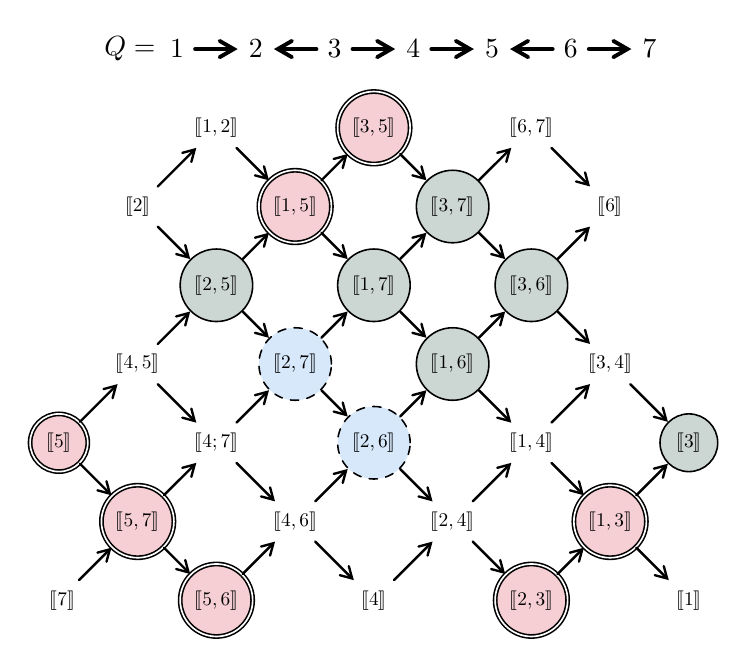
\begin{tikzpicture}
				\begin{scope}[line width=.5mm,->, >= angle 60]
                    \node at (-.6,0){$Q=$};
					\node (a) at (0,0){$1$};
					\node (b) at (1,0){$2$};
					\node (c) at (2,0){$3$};
					\node (d) at (3,0){$4$};
                    \node (e) at (4,0){$5$};
                    \node (f) at (5,0){$6$};
                    \node (g) at (6,0){$7$};
					\draw (a) -- (b);
					\draw (c) -- (b);
					\draw (c) -- (d);
                    \draw (d) -- (e);
                    \draw (f) -- (e);
                    \draw (f) -- (g);
				\end{scope}
                \begin{scope}[yshift=-2cm, xshift=-.5cm, line width=.3mm, ->, >= angle 60]
					\node (2) at (0,0){\scalebox{.7}{$\llrr{2}$}};
					\node (12) at (1,1){\scalebox{.7}{$\llrr{1,2}$}};
					\node[circle,line width=0.2mm,fill=darkgreen!20,draw] (2345) at (1,-1){\scalebox{.7}{$\llrr{2,5}$}};
					\node (45) at (0,-2){\scalebox{.7}{$\llrr{4,5}$}};
                    \node[circle,line width=0.2mm,double,fill=lava!20,draw] (5) at (-1,-3){\scalebox{.7}{$\llrr{5}$}};
                    \node[circle,line width=0.2mm,double,fill=lava!20,draw] (567) at (0,-4){\scalebox{.7}{$\llrr{5,7}$}};
                    \node (7) at (-1,-5){\scalebox{.7}{
							$\llrr{7}$}};
                    \node (56)[circle,line width=0.2mm,double,fill=lava!20,draw] at (1,-5){\scalebox{.7}{$\llrr{5,6}$}
                                };
                     \node (4) at (3,-5){\scalebox{.7}{$\llrr{4}$}};
                     \node[circle,line width=0.2mm,double,fill=lava!20,draw] (23) at (5,-5){\scalebox{.7}{$\llrr{2,3}$}};
                    \node (1) at (7,-5){\scalebox{.7}{$\llrr{1}$}};
                    \node (456) at (2,-4){\scalebox{.7}{$\llrr{4,6}$}};
                    \node (234) at (4,-4){\scalebox{.7}{$\llrr{2,4}$}};
                     \node[circle,line width=0.2mm,double,fill=lava!20,draw] (123) at (6,-4){\scalebox{.7}{$\llrr{1,3}$}};
                     \node (4567) at (1,-3){\scalebox{.7}{$\llrr{4;7}$}};
                     \node[circle,line width=0.2mm,dashed,fill=bleudefrance!20,draw] (23456) at (3,-3){\scalebox{.7}{$\llrr{2,6}$}};
                     \node (1234) at (5,-3){\scalebox{.7}{$\llrr{1,4}$}};
                     \node[circle,line width=0.2mm,fill=darkgreen!20,draw] (3) at (7,-3){\scalebox{.7}{$\llrr{3}$}};
					\node[circle,line width=0.2mm, double,fill=lava!20,draw] (12345) at (2,0){\scalebox{.7}{$\llrr{1,5}$}};
					\node[circle,line width=0.2mm, dashed,fill=bleudefrance!20,draw] (234567) at (2,-2){\scalebox{.7}{$\llrr{2,7}$}};
                    \node[circle,line width=0.2mm,fill=darkgreen!20,draw] (123456) at (4,-2){\scalebox{.7}{$\llrr{1,6}$}};
					\node (34) at (6,-2){\scalebox{.7}{$\llrr{3,4}$}};
					\node[circle,line width=0.2mm,fill=darkgreen!20,draw] (1234567) at (3,-1){\scalebox{.7}{$\llrr{1,7}$}};
                    \node[circle,line width=0.2mm,fill=darkgreen!20,draw] (3456) at (5,-1){\scalebox{.7}{$\llrr{3,6}$}};
                    \node[circle,line width=0.2mm,fill=darkgreen!20,draw] (34567) at (4,0){\scalebox{.7}{$\llrr{3,7}$}};
                    \node (6) at (6,0){\scalebox{.7}{$\llrr{6}$}};
                    \node[circle,line width=0.2mm,double,fill=lava!20,draw] (345) at (3,1){\scalebox{.7}{$\llrr{3,5}$}};
                    \node (67) at (5,1){\scalebox{.7}{$\llrr{6,7}$}};
					\draw (2) -- (12);
					\draw (2) -- (2345);
					\draw (45) -- (2345);
					\draw (12) -- (12345);
					\draw (2345) -- (12345);
					\draw (2345) -- (234567);
                    \draw (12345) -- (345);
                    
                    
                    \draw (5) -- (45);
                    \draw (7) -- (567);
                    \draw (567) -- (4567);
                    \draw (4567) -- (234567);
                    \draw (234567) -- (1234567);
                    \draw (1234567) -- (34567);
                    \draw (34567) -- (67);
                    \draw (56) -- (456);
                    \draw (456) -- (23456);
                    \draw (23456) -- (123456);
                    \draw (123456) -- (3456);
                    \draw (3456) -- (6);
                    \draw (4) -- (234);
                    \draw (234) -- (1234);
                    \draw (1234) -- (34);
                    \draw (23) -- (123);
                    \draw (123) -- (3);
					
					\draw (5) -- (567);
                    \draw (567) -- (56);
                    \draw (45) -- (4567);
                    \draw (4567) -- (456);
                    \draw (456) -- (4);
                    \draw (234567) -- (23456);
                    \draw (23456) -- (234);
                    \draw (234) -- (23);
                    \draw (12345) -- (1234567);
                    \draw (1234567) -- (123456);
                    \draw (123456) -- (1234);
                    \draw (1234) -- (123);
                    \draw (123) -- (1);
                    \draw (345) -- (34567);
                    \draw (34567) -- (3456);
                    \draw (3456) -- (34);
                    \draw (34) -- (3);
                    \draw (67) -- (6);	
				\end{scope}
    \end{tikzpicture} 
    
\end{frame}







\begin{frame}{Nice Properties of \(\GS_\mathcal{E}\)}
\emph{\begin{block}{Proposition}
Let $\mathscr{C} \subseteq \mathscr{A}$ be a subcategory.
\begin{enumerate}[label=(\arabic*), itemsep=2mm]
\pause
  \item If $\mathscr{C}$ is $\mathcal{E}$-adapted, then $\GS_\mathcal{E}(\mathscr{C})$ is also $\mathcal{E}$-adapted.
\pause

  \item If $\mathscr{C}$ is $\mathcal{E}$-adapted and extension-closed, then $\GS_\mathcal{E}(\mathscr{C})$ is also extension-closed.
\end{enumerate}
\end{block}

\bigskip


\pause
\textbf{Corollary 1.}
Let $T \in \mathscr{A}$ be a tilting object.  
Then $\GS_\mathcal{E}(T)$ is $\mathcal{E}$-adapted and extension-closed.

\bigskip
\pause
\textbf{Corollary 2.}
Let $T \in \text{rep}(A_n)$ be a tilting object.  
Then $\GS_\mathcal{E_\diamond}(T)$ is canonically Jordan recoverable.
}

\bigskip
\pause
\textbf{Question}: Is $\GS_\mathcal{E_\diamond}(T)$ maximal canonically Jordan recoverable?



\end{frame}




\begin{frame}{First Main Theorem}
\begin{theorem} [Dequêne–R, 2025]
Let $T \in \mathscr{A}$ be a tilting object.  
Then $\GS_\mathcal{E}(T)$ is a maximal $\mathcal{E}$-adapted, extension-closed subcategory of $\mathscr{A}$ containing $T$.
\end{theorem}
\pause
\bigskip



\emph{In particular, every maximal canonically Jordan recoverable subcategory arises as 
\(\GS_{\mathcal{E}_\diamond}(T)\) for some tilting object $T$.}
\pause
\begin{block}{Corollary}
For any tilting object \(T \in \mathscr{A}\),
\[
\GS_{\mathcal{E}}(T)
\;=\;
\GS_{\mathcal{E}}^2(T).
\]
\end{block}
\bigskip
\pause
How can we describe the equivalence relation :
\[ T \sim_\mathcal{E} T' \iff \GS_{\mathcal{E}}(T) = \GS_{\mathcal{E}}(T') \text{?}
  \]
\end{frame}

\section{Relative Mutations \& Tilting Equivalence\\ \normalsize (Second Main Theorem)}
\begin{frame}{Classical and Relative Mutation}


\emph{\begin{block}{Definition} 
Let $T = U \oplus \overline{T}$ be a tilting object with $U$ indecomposable.  

\begin{itemize}
  \item A \textbf{mutation} of $T$ at $U$ is a tilting object
  \[
  \mu_U(T) \;=\; U' \oplus \overline{T},
  \]
  where $U'$ is an indecomposable object obtained from $U$ by an \emph{exchange sequence}
 \[
  \xi:\;
  0 \rightarrow 
  U \xrightarrow{f} B \xrightarrow{g} U' \rightarrow 0 
  \;,
  \qquad 
  B \in \add(\overline{T}),
  \]
  where \\
  $f$ \text{ is a left minimal } \add(\overline{T})\text{-approximation of } $U$,
  \\
  $\;\;\;\;g$ \text{ is a right minimal } \add(\overline{T})\text{-approximation of } $U'$.
  \end{itemize}
  \end{block}
  }
\pause
   We write \(\mu_U^+(T)\) (resp. \(\mu_U^-(T)\)) for the \emph{right} (resp. \emph{left}) mutation.


\end{frame}

\begin{frame}{Classical and Relative Mutation}
\emph{\begin{block}{Definition} 
Let $T = U \oplus \overline{T}$ be a tilting object with $U$ indecomposable.  

\begin{itemize}
  \item An \textcolor{blue}{$\mathcal{E}$}-\textbf{mutation} of $T$ at $U$ is a tilting object
  \[
  \mu_U(T) \;=\; U' \oplus \overline{T},
  \]
  where $U'$ is an indecomposable object obtained from $U$ by an \textcolor{blue}{$\mathcal{E}$}-\emph{exchange sequence}
  \[
  \xi:\;
  0 \rightarrow 
  U \xrightarrow{f} B \xrightarrow{g} U' \rightarrow 0 
  \;\in\; \textcolor{blue}{\mathcal{E}},
  \qquad 
  B \in \add(\overline{T}),
  \]
  where \\
  $f$ \text{ is a left minimal } \add(\overline{T})\text{-approximation of } $U$,
  \\
  $\;\;\;\;g$ \text{ is a right minimal } \add(\overline{T})\text{-approximation of } $U'$.
  \end{itemize}
  \end{block}
  }
  We write \(\mu_{U,\textcolor{blue}{\mathcal{E}}}^+(T)\) (resp. \(\mu_{U,\textcolor{blue}{\mathcal{E}}}^-(T)\)) for the \emph{right} (resp. \emph{left}) \textcolor{blue}{$\mathcal{E}$}-mutation.


\end{frame}


\begin{frame}{Example : 
$Q = 1 \rightarrow 2 \leftarrow 3 \rightarrow 4$ with $\mathcal{E}=\mathcal{E_{\text{max}}}$ 
}
\centering

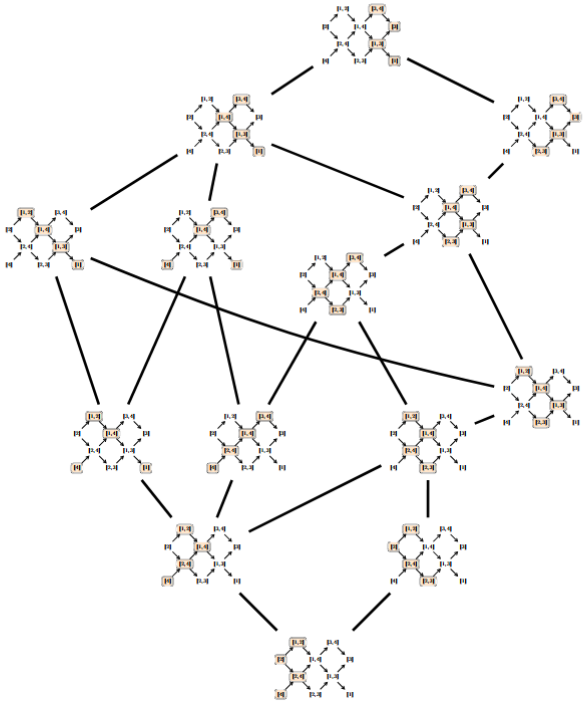
\includegraphics[width=0.6\textwidth]{poset_A4_Ediamond.png}
\end{frame}



\begin{frame}{\(\mathcal{E}\)-Reachability}

 \emph{\begin{block}{Definition}
Let \(T,T'\in\Tilt(Q)\).
\pause


   \(T'\) is \textbf{\(\mathcal{E}\)-reachable} from \(T\)  if there exist indecomposables \((U_1,\dots,U_m)\) such that
  \[
  T' \cong \mu_{U_m,\mathcal{E}}\circ\cdots\circ \mu_{U_1,\mathcal{E}}(T).
  \]




\end{block}
}
\pause
\textbf{\(\mathcal{E}\)-reachability} : $T \approx_{\mathcal{E}} T'$ forms a equivalence relation. We denote $[T]_{\approx_\mathcal{E}}$ for the equivalence class of $T$.


\end{frame}


\begin{frame}{Example : 
$Q = 1 \rightarrow 2 \leftarrow 3 \rightarrow 4$ with $\mathcal{E}=\mathcal{E_\diamond}$
}
\centering

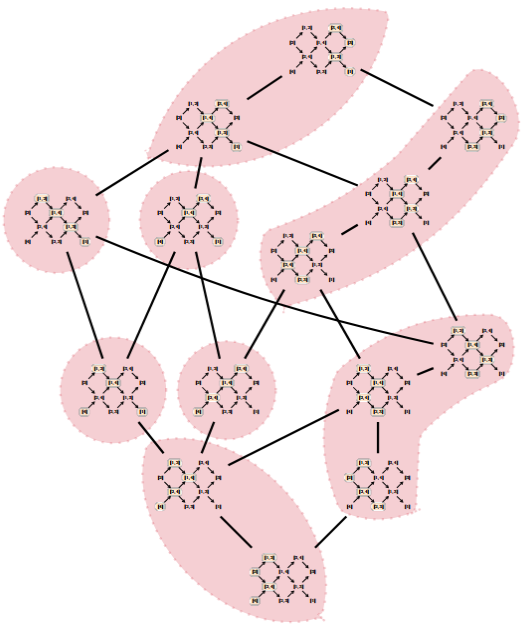
\includegraphics[width=0.6\textwidth]{poset_A4_Ediamond_pink.png}
\end{frame}



\begin{frame}{Equivalence of Tiltings}

    

\emph{ \begin{block}{Proposition}
    
Let $T,T' \Tilt(Q)$.  
Then \[
T \sim_{\mathcal{E}} T'
\quad \Longleftrightarrow \quad
T \approx_{\mathcal{E}} T'.
\]
\end{block}
\pause
\textbf{Example.} Assume $Q = 1 \rightarrow 2 \leftarrow 3 \rightarrow 4$ and $\mathcal{E}=\mathcal{E_\diamond}$.

\bigskip
\pause

$\;\;\;\;[T_1]_{\approx_{\mathcal{E}_\diamond}}=[T_2]_{\approx_{\mathcal{E}_\diamond}}=[T_3]_{\approx_{\mathcal{E}_\diamond}} \;\;\;\;\; \only<4->{\GS_\mathcal{E_\diamond}(T_1) =
\GS_\mathcal{E_\diamond}(T_2) = \GS_\mathcal{E_\diamond}(T_3)}
$

\begin{columns}
  \column{0.35\textwidth}
  \centering
  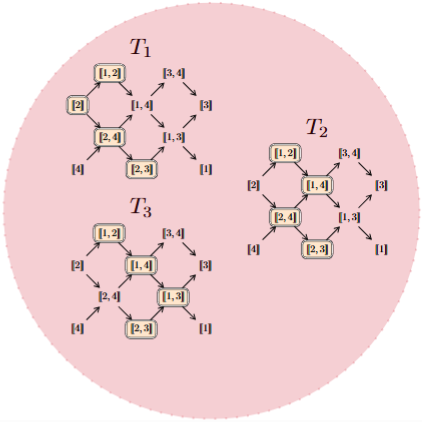
\includegraphics[width=\textwidth]{OneClass.png}
\pause
  \column{0.35\textwidth}
  \centering
  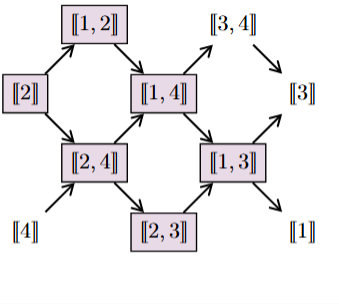
\includegraphics[width=\textwidth]{GSA4.png}
\end{columns}


}
\end{frame}





\begin{frame}{Second Main Theorem}
\begin{theorem}[Dequêne–R, 2025]
Let $T \in \Tilt(Q)$. Then
\[
\GS_{\mathcal{E}}(T)
\;=\;
\add \left( \bigoplus_{T' \in [T]_{\approx_{\mathcal{E}}}} T' \right).
\]
\end{theorem}

\pause

\textbf{Example.} Assume $Q = 1 \rightarrow 2 \leftarrow 3 \rightarrow 4$ and $\mathcal{E}=\mathcal{E_\diamond}$.
\smallskip
\pause

\centering
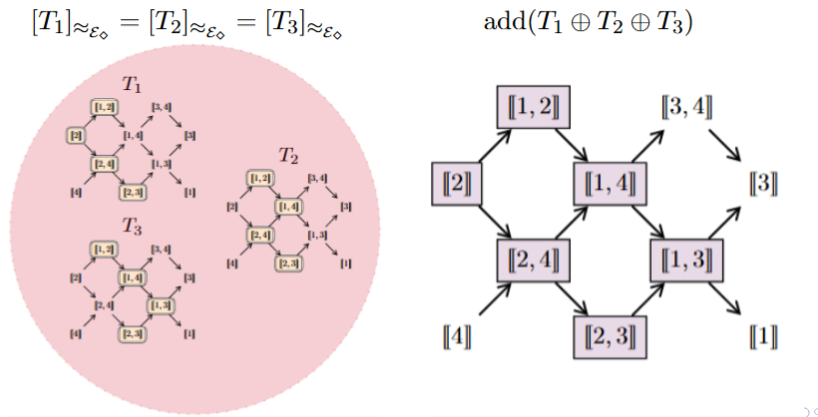
\includegraphics[width=0.7\textwidth]{addA4.png}

\end{frame}






\begin{frame}{Consequences of the Second Main Theorem}
\begin{corollary} Let $Q$ be a quiver of type $A_n$.
\pause
\begin{enumerate}[label=(\alph*), itemsep=3mm]
    \item There is a bijection
   \[
       \Tilt(Q) / {\approx_{\mathcal{E}_\diamond}}
       \;\longleftrightarrow\;
       \text{\{maximal \text{CJR} subcategories of }\rep(Q)\}.
    \]
    \pause
    \item Let $\mathscr{C} \subseteq \rep (Q)$ be a maximal canonically Jordan recoverable subcategory. Then there exists $T \in \Tilt(Q)$ such that \[\mathscr{C} = \add \left( \bigoplus_{T' \in [T]_{\approx_{\mathcal{E}_\diamond}}} T' \right). \]
    
\end{enumerate}
\end{corollary}
\end{frame}
\begin{frame}{Synthesis and Outlook}


\textbf{A unified picture of exact structures and recoverability}\\[0.8em]


\pause
\begin{itemize}
  \item The \textcolor{blue}{diamond exact structure} $\mathcal{E}_\diamond$ provides a natural framework 
  connecting tilting theory and Jordan recoverability.
  \pause

  \item Every maximal canonically Jordan recoverable subcategory 
  emerges as $\GS_{\mathcal{E}_\diamond}(T)$ for some tilting object~$T$.
  \pause

  \item Two tilting objects $T, T'$ satisfy 
  \(\GS_{\mathcal{E}}(T) = \GS_{\mathcal{E}}(T')\)
  if and only if they are related by a sequence of 
  $\mathcal{E}$-\textcolor{blue}{mutations}.
  \pause

  \item
  There is a bijection
  \[
    \mathrm{Tilt}(Q)/{\approx_{\mathcal{E}_\diamond}}
    \;\longleftrightarrow\;
    \{\text{maximal CJR subcategories of }\rep(Q)\},
  \]
  given by 
  \[
     [T]_{\approx_\mathcal{E_\diamond}} \;\longmapsto\;
    \add\!\Bigl(\!\bigoplus_{T' \in [T]_{\approx_{\mathcal{E}_\diamond}}} T'\Bigr).
  \]
\end{itemize}

\vfill
\pause
\begin{center}
\textit{Thank you for listening.}\\[0.3em]
\small Based on joint work with Benjamin Dequêne (arXiv:2509.25012)
\end{center}
\end{frame}

\begin{frame}[plain]
    \centering
    \vfill
    {\Huge \textbf{Thank you for listening!}} \\[1cm]
    {\Large Questions?}
    \vfill
    \centering


\includegraphics[width=0.6\textwidth]{logo_frq_1920x1080px_fond_blanc-768x432.jpg}
\end{frame}
\end{document}

